\chapter{Scene Graphs, Node Transforms and State Machines}
In this chapter we will implement the catching mechanism for our game. This will
require you to learn more details about scene graphs, node transforms and also about modelling game mechanics in Swift.

You will learn how to incorporate state machines into games. You will also learn
how to detect if objects have been caught or not and how to manipulate the
scene graph make objects fall into our catching pot.

There's lots of work ahead of us!

\section{Catching Objects}
Implementing drag and drop was a great warm up. In this section we are going to
solve a bunch of problems that will bring our little project a large step closer
to being a real game. By the end of this section the user will be able to catch
and miss objects by dragging the pot with the right timing.

Before we dive into coding let's think about what we actually need to implement.
There are three important aspects that need to be covered through our
implementation:
\begin{enumerate}
  \item detecting if the user has caught an object
  \item detecting if the user has missed an object
  \item visualizing catching / missing correctly
\end{enumerate}

\subsection{Thinking in States}
Our feature outline describes that objects start out as falling objects,
directly after they have been spawned. At some later point in time the user can
catch or miss these objects. In each of these situations we need our falling objects to behave differently. If they are
falling we want them to move down the screen with a constant speed. If they are
caught we need some sort of visualisation - ideally the objects move into the
pot and disappear. If the user tries to catch an object too late and misses it
closely we want to visualize that, too.

From the paragraph above we can extract three different states in which a
falling object can be:
\begin{figure}[H]
		\centering
		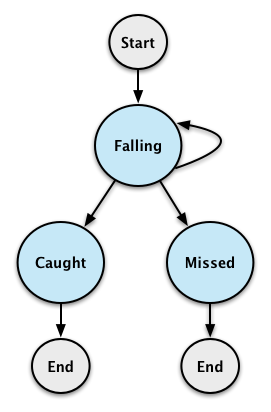
\includegraphics[width=0.3\linewidth]{images/Chapter3/falling_object_states.png}
		\caption{Objects start in falling state, then they end up caught or missed}
\end{figure}
As the diagram shows, a falling object can either stay a falling object or turn
into a caught or missed object. It is up to us developers to decide the criteria
for a state change. We also need to decide when we want to check for state
changes.

For our game I suggest that we check whether a player has caught an object or
not in the \inlinecode{update} method. As soon as that object reaches the y
position of the top of the pot we decide based on the x position whether the
object has been caught or missed 
\begin{figure}[H]
		\centering
		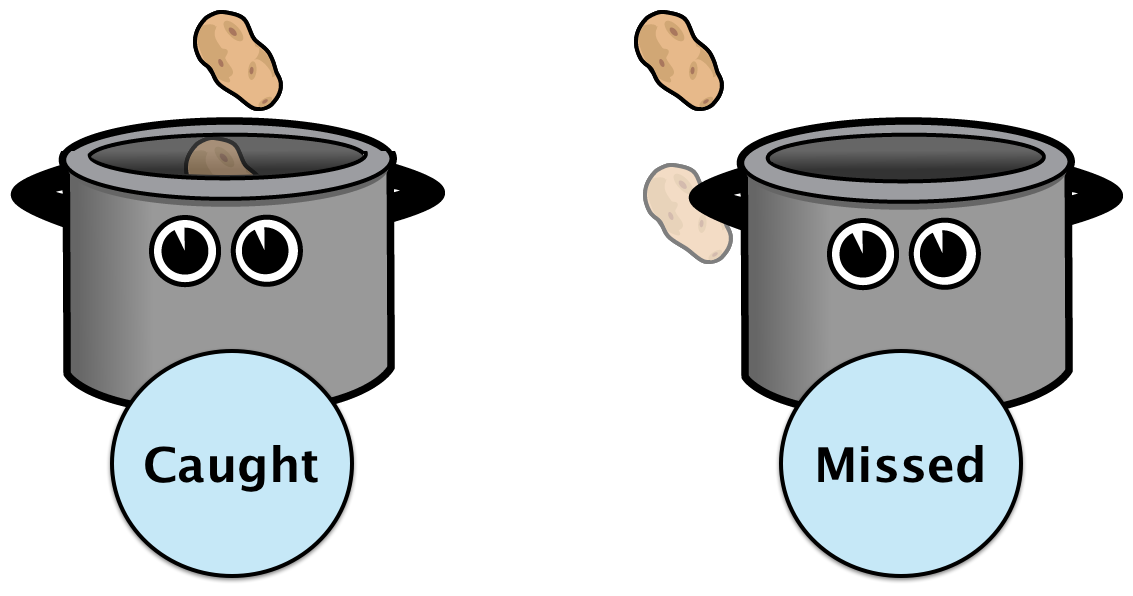
\includegraphics[width=0.3\linewidth]{images/Chapter3/catch_test.png}
		\caption{Caught objects fall into the pot, missed objects fall behind}
		\label{CaughtMissedDefinition}
\end{figure}
Since we are building a 2D game we only have limited ways of expressing that a
player missed a falling object - I suggest that we render missed objects behind
the pot. That way players can quickly see whether they caught an object or not.

Now we have a good starting point for some coding; we need to store
different states for falling objects and we need to write specific behavior
code for each of these states. Additionally we need to write code that checks if
we have caught or missed an object so that we can assign the correct states to
falling objects.

\subsection{Storing State}
Now it's time to implement the theoretical conctepts that we've discussed. 
Let's start by adding a \inlinecode{fallingState} to
\inlinecode{FallingObject.swift}. That state variable will remember whether an object is currently falling, has been caught
or has been missed.

The best way to represent states in Swift is to use an enumeration!
\begin{leftbar}
Add this enum definition to \inlinecode{FallingObject.swift} below the
\inlinecode{FallingObjectType} enum:
\begin{lstlisting}
  enum FallingObjectState {
    case Falling
    case Caught
    case Missed
  }
\end{lstlisting}
\end{leftbar}
As mentioned earlier, associating enum entries with a type is not
mandatory. In this case our entries don't need a type (e.g. Int) since the
entries will only represent a state - they are values in their own right.

\begin{leftbar}
Next, add a property to store the current state:
\begin{lstlisting}
  var fallingState = FallingObjectState.Falling
\end{lstlisting}
\end{leftbar}
This variable should not be private, we want to change the value as
the object gets caught or missed. Our default state is \inlinecode{.Falling}, we
assign it as part of the variable declaration.

Now we can store a \inlinecode{fallingState} for each falling object; next,
let's implement different behaviour based on that state.

\subsection{Implement State Specific Behaviour}
The majority of our gameplay code is currently inside of the \inlinecode{update}
method of \inlinecode{MainScene}. This is fairly common for simple games.
Currently we are doing two things in the update method: moving the objects down
the screen and checking whether they have left the stage entirely (in which
case we delete them). Now however, we are going to add code that will only run
for falling objects in certain states. That will add quite a lot of complexity.
Instead of squashing everything into the update method I suggest that we
create one method for each of the three states. These methods will contain
all state specific code and will be called from within the \inlinecode{update}
method.

\begin{leftbar}
Replace your existing update method with the following one:
\begin{lstlisting}
    override func update(delta: CCTime) {
    // use classic for loop so that we can remove objects while iterating over the array
    for (var i = 0; i < fallingObjects.count; i++) {
      let fallingObject = fallingObjects[i]
      
      // let the object fall with a constant speed
      fallingObject.position = ccp(
        fallingObject.position.x,
        fallingObject.position.y - CGFloat(fallingSpeed * delta)
      )
      
      switch fallingObject.fallingState {
      case .Falling:
        performFallingStep(fallingObject)
      case .Missed:
        performMissedStep(fallingObject)
      case .Caught:
        performCaughtStep(fallingObject)
      }
    }
  }
\end{lstlisting}
\end{leftbar} 
Now the update method is really easy to read. We loop over all falling objects.
In all cases we move the falling object towards the bottom of the screen. After
that we check in which state an object is and invoke a method that contains code
specific to that state. We are going to implement these methods throughout the
remainder of this chapter.

\subsection{Implementing the Falling State}
Let's start implementing the default state: falling. In this state we will need
check whether an object has been caught, has been missed or simply remains
falling. 

In figure \ref{CaughtMissedDefinition} we have illustrated what we consider a
caught/missed object. So how can we implement this? Basically all we need to do
is compare the frame of the falling object to the frame of the pot. However,
there is one small issue. The frame of a \ccsprite{} is always a rectangle that
encloses the entire texture. Here's what the dimensions of the frames of our pot
and a falling object look like:
\begin{figure}[H]
		\centering
		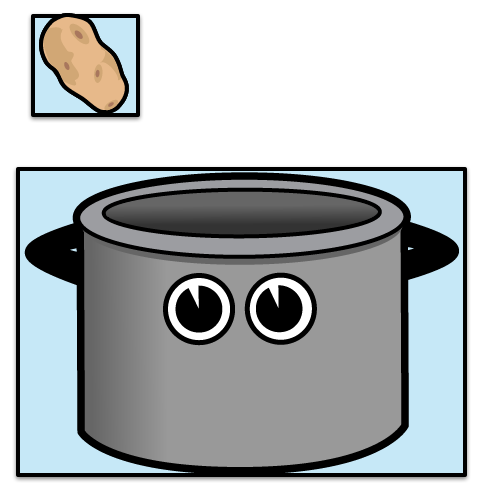
\includegraphics[width=0.3\linewidth]{images/Chapter3/frame_pot_falling_object.png}
		\caption{The pot frame is too large to use it for collision detection}
\end{figure}
From the illustration above you can see that the frame of the pot is too large
to use it for collision detection. It could easily happen that an object
landing on the handle of the pot would still be considered a catch.

Instead of using the pot dimensions we will need to add a separate, smaller,
node in \SB{} that marks the catch area. 
\begin{leftbar}
Open the \SB{} project and open \filemention{Pot.ccb}
\begin{figure}[H]
		\centering
		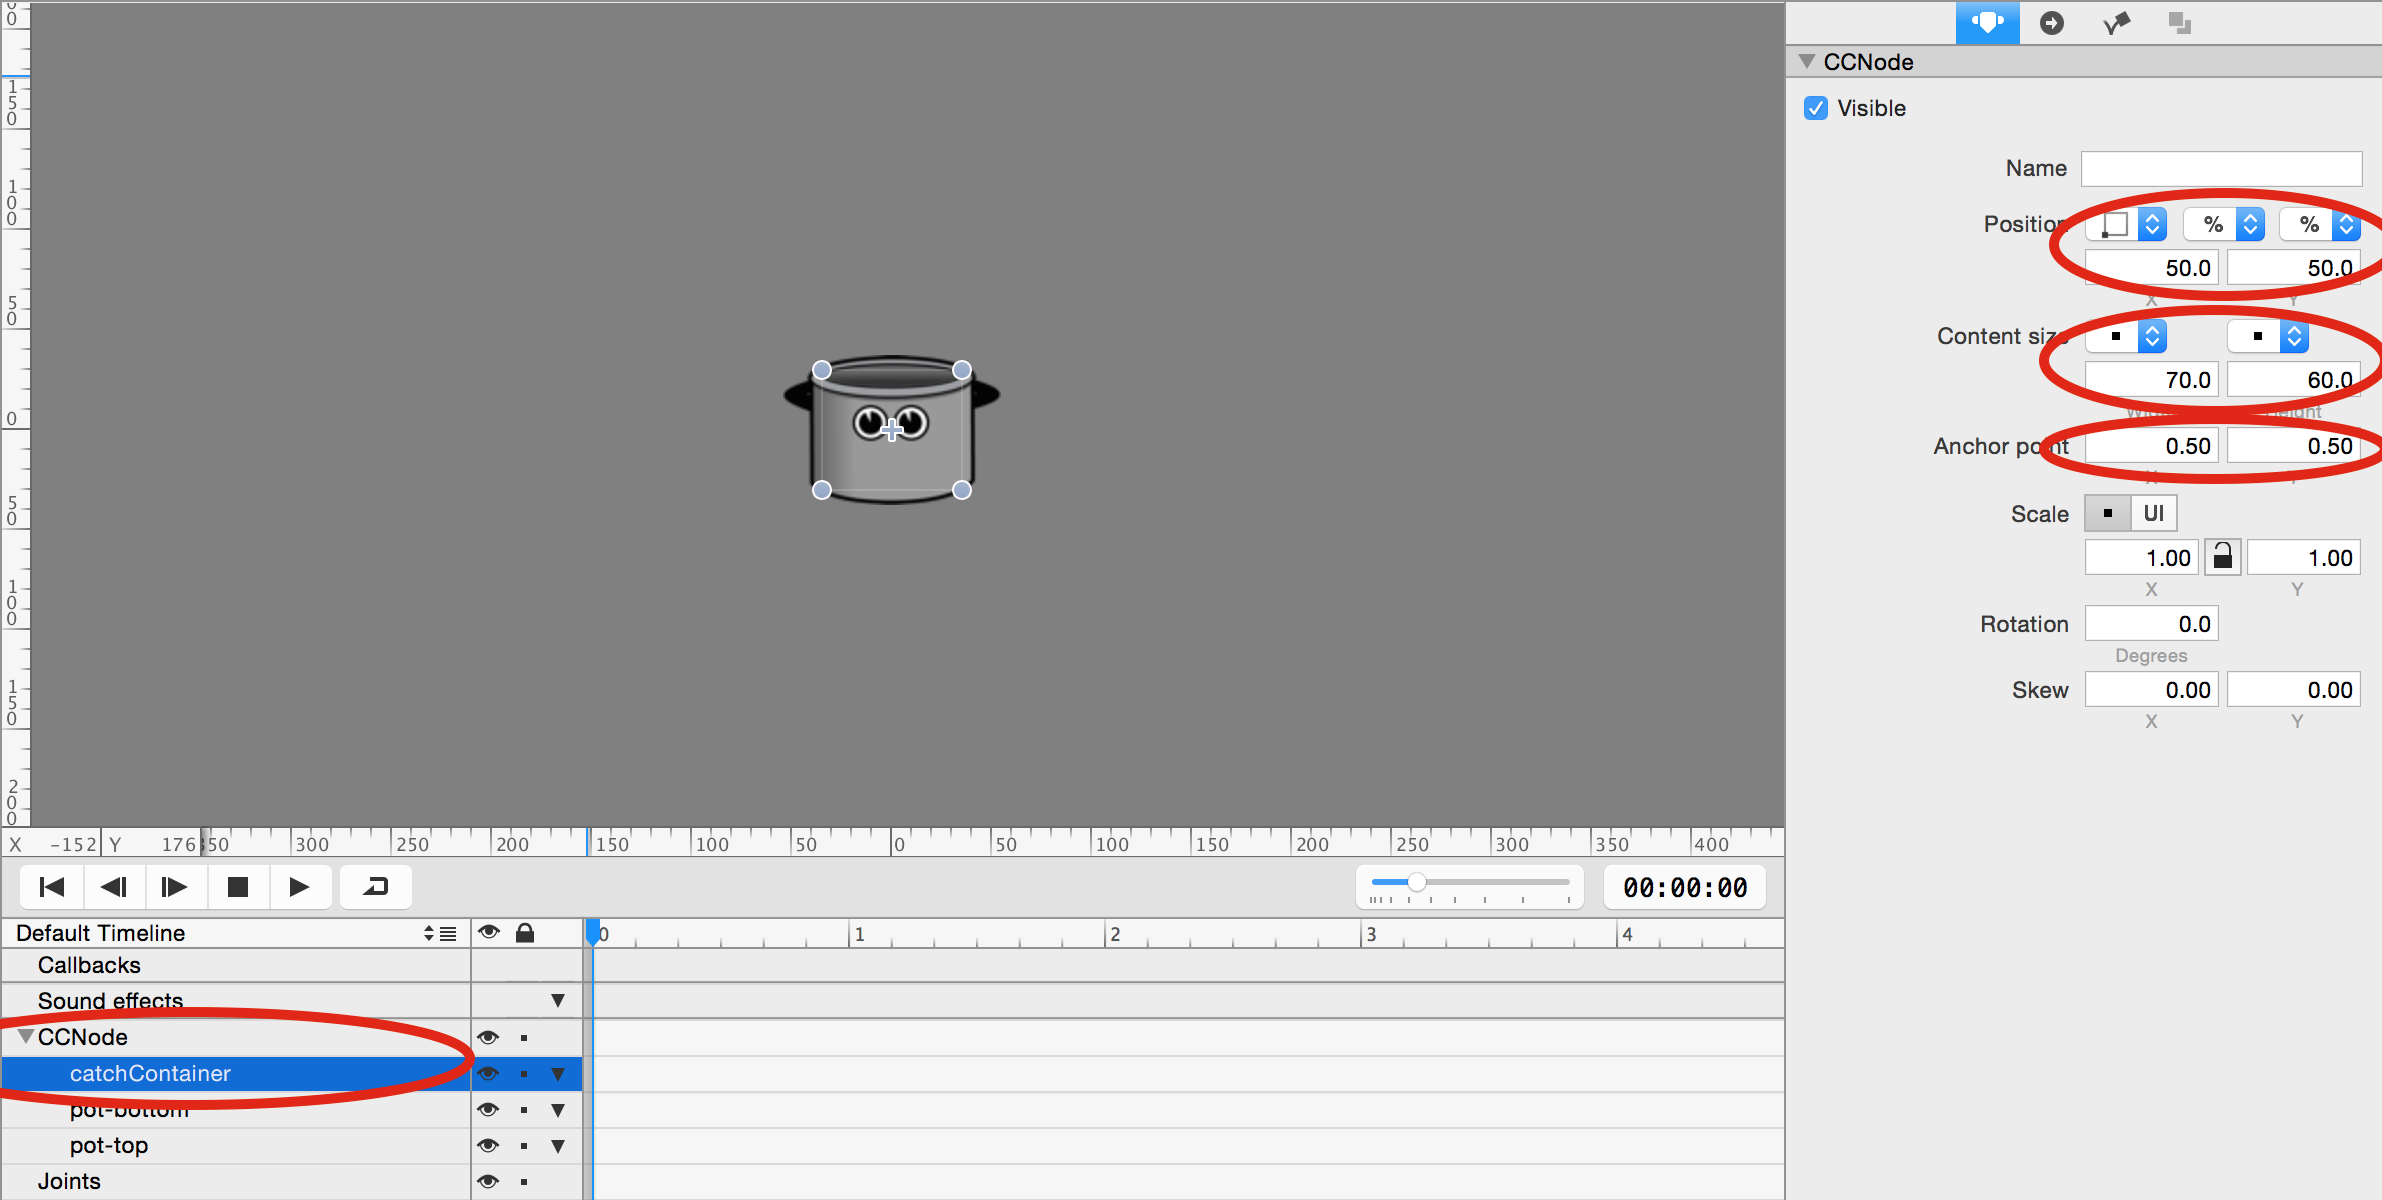
\includegraphics[width=0.8\linewidth]{images/Chapter6/add_catch_container_2.png}
		\caption{The size and position of this container will determine when objects
		are caught / missed}
\end{figure}

\begin{enumerate}
  \item Add a plain \textit{Node} from the node library and add it as a child to
root node, as highlighted in the screenshot above. A short
reminder: the easiest way to do this, is dragging the node from the node library
into the timeline and dropping it on top of \textit{pot-bottom} node.
  \item Set up \textit{Position Type}, \textit{Position} and \textit{Anchor
  Point} of the container, as shown in the image above
  \item Because we want to reference this catch container in code you will need to set a
code connection, too. Set the target to \textit{Doc root var} and call the
variable \inlinecode{catchContainer}:
\begin{figure}[H]
    \centering
    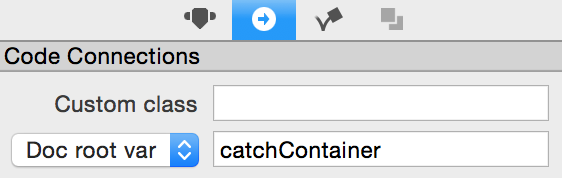
\includegraphics[width=150pt]{images/Chapter6/container_cc.png}
\end{figure}
  \item Since the container is now connected to the root
  node of \filemention{Pot.ccb}, through the \inlinecode{catchContainer}
  property, the root node needs a custom class that has that property. Select
  the root node and set the custom class to \inlinecode{Pot}
\begin{figure}[H]
    \centering
    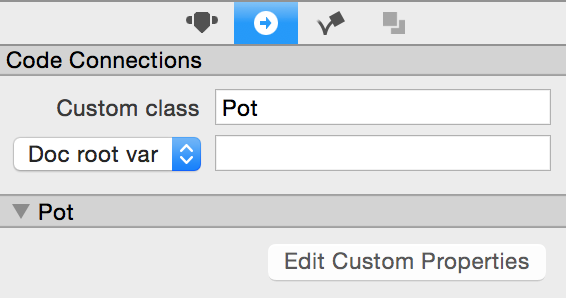
\includegraphics[width=150pt]{images/Chapter6/pot_cc.png}
\end{figure}
\item Publish the \SB{} project
\end{enumerate}
\end{leftbar}

Next, we need to create the \inlinecode{Pot} class that we just referenced,
along with its \inlinecode{catchContainer} property!

\begin{leftbar}
\begin{enumerate}
  \item Create a new Class in \xcode{} and name it \filemention{Pot}. Make it a
  subclass of \ccnode{}
  \item Add the \inlinecode{catchContainer} property so that the class
  definition looks like this:
  \begin{lstlisting}
  class Pot: CCNode {
  
    weak var catchContainer: CCNode!
  
  }
  \end{lstlisting}
\end{enumerate}
\end{leftbar}
Now we have a reference container set up. That container will allow us to test
if objects have been caught or dropped. Remember, all of this code will taking
place in the \textit{falling step} state. 

We can now start implementing falling step method.
\begin{leftbar}
Add the method stub for the falling step to \filemention{MainScene.swift}:
\begin{lstlisting}
  func performFallingStep(fallingObject:FallingObject) {

  }
\end{lstlisting}
\end{leftbar}
Before we can dive into collision detection we will have to take a little detour
and talk about node transformations.\index{Node transformation!Bounding Box} As
part of the introduction to \cocos{} we have discussed that nodes are always positioned
relative to their parent node (chapter: \ref{Introduction_CCNode}). The catch
container that we just added in \SB{} is a child of the \inlinecode{Pot}
node. We chose that setup so that the catch container always moves together
with the pot. 

For our collision detection algorithm we want to compare the position of a
falling object to the position of our catch container. \textbf{Here the problem
arises: falling objects and the catch container have different parent nodes,
that means we cannot compare their positions and frames directly.} Since the
position is relative to the parent node, comparing nodes with different parents
would resolve in unexpected behavior. Take the following illustration as an
example:
\begin{figure}[H]
		\centering
		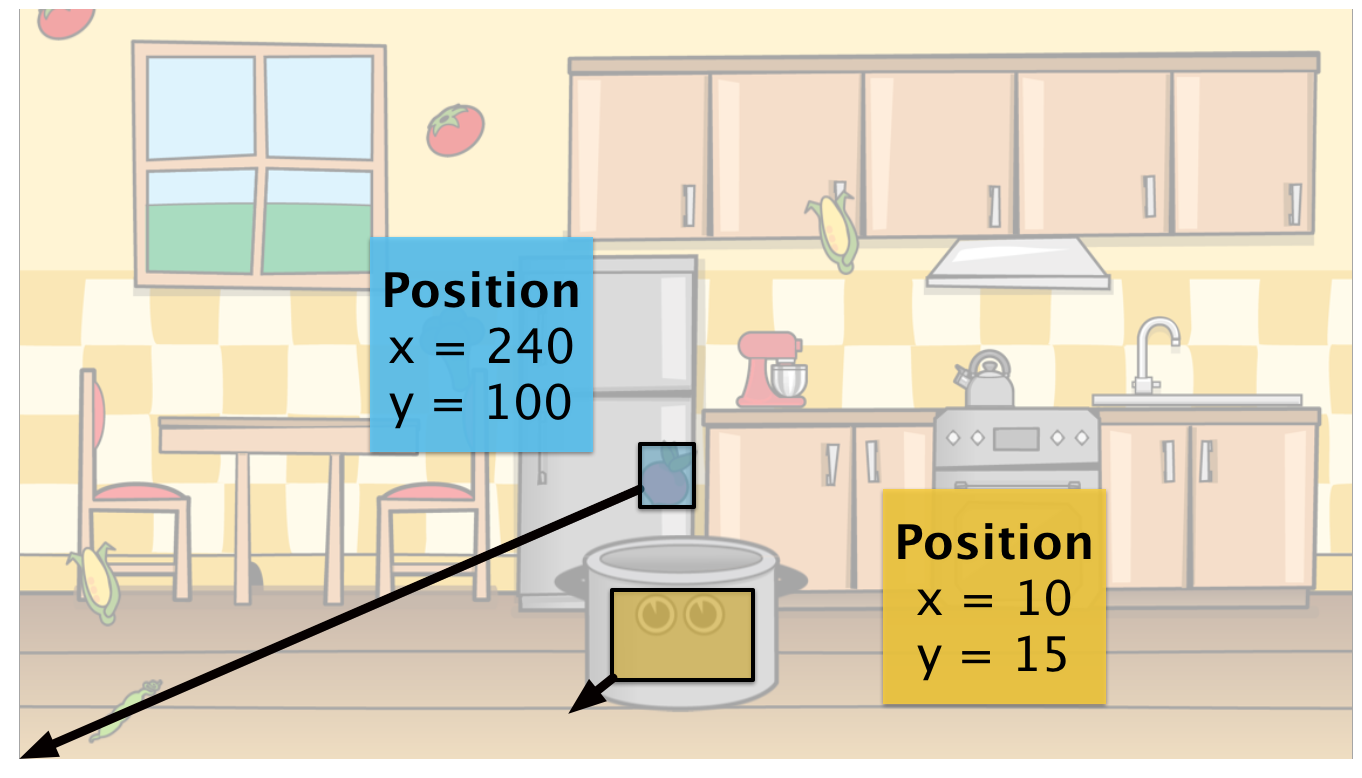
\includegraphics[width=0.7\linewidth]{images/Chapter3/parent_transform.png}
		\caption{Even though the two nodes illustrated above are close to each other,
		their position values are entirely different, since they are placed relative
		to different parents}
\end{figure}
How can we work around this? Luckily \cocos{} exposes a couple of variables and
methods that allows us to transform positions and frames between different
\textit{node spaces}. Each node lives in the \textit{node space} of its parent.
In our example the catch container is in the node space of the pot and the pot is
in the node space of the main scene.

If we want to know the position and size of the catching container in the main
scene node space, we need to apply the following transform:
\begin{lstlisting}
let containerWorldBoundingBox = CGRectApplyAffineTransform(
  catchContainer.boundingBox(), catchContainer.parent.nodeToParentTransform()
);
\end{lstlisting}
We are transforming the bounding box of the catch container using the
\inlinecode{nodeToParentTransform} of the catch container's parent node (the
pot). The \cocos{} documentation describes the
\inlinecode{nodeToParentTransform} as following: \textit{Returns the matrix that
transform the node's (local) space coordinates into the parent's space coordinates.}

This means after applying the transform we know the position of the catch
container in the main scene space. With the dimensions of both nodes in the same
space, we can perform the bounding box comparison.

If you are new to graphics programming this concept will likely seem a little
confusing; frankly you won't need it too often when working with \cocos{}. If
you aren't getting a hold of transforms yet, don't worry about it!

\begin{details}[The role of transforms in graphics programming]
Transforms are an essential part of all graphics engines - also of \cocos{}.
When determining the positions for all nodes in a scene, \cocos{} starts with
the root node. After the root node is laid out, the engine moves to the children
of the root node, calculates their position and places them \textit{relative to
the root node}. This is repeated all the way down the node hierarchy:
\begin{figure}[H]
		\centering
		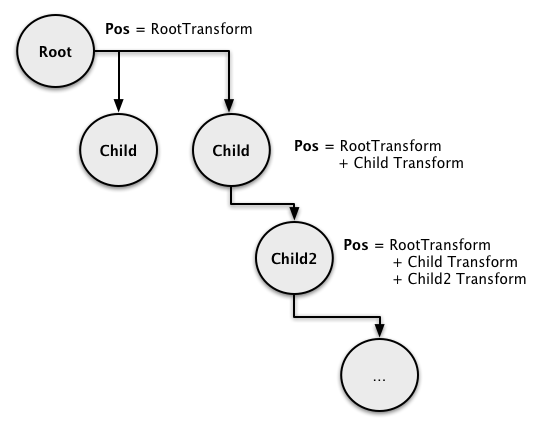
\includegraphics[width=0.5\linewidth]{images/Chapter3/parent_transform_rendering.png}
\end{figure}
\end{details}

Now that we have a solution for the transformation issue, the rest of the
code that we need for the falling step is not too complicated.

First, change the type of our \inlinecode{pot} property from \ccsprite to
\inlinecode{Pot} so that we can access the \inlinecode{catchingContainer}
property from within \inlinecode{MainScene}.

\begin{leftbar}
Change the code connection property \inlinecode{pot} within
\filemention{MainScene.swift} to look like this:
\begin{lstlisting}
  weak var pot: Pot!
\end{lstlisting}
\end{leftbar}

Now we can implement the falling step method! Let's first add the code and then
discuss it in detail.

\begin{leftbar}
Replace the \inlinecode{performFallingStep} stub with this implementation:
\begin{lstlisting}
  func performFallingStep(fallingObject:FallingObject) {
    let containerWorldBoundingBox = CGRectApplyAffineTransform(
      pot.catchContainer.boundingBox(), pot.nodeToParentTransform()
    );
    
    let yPositionInCatchContainer = CGRectGetMinY(fallingObject.boundingBox()) < CGRectGetMaxY(containerWorldBoundingBox)
    let xPositionLargerThanLeftEdge = CGRectGetMinX(fallingObject.boundingBox()) > CGRectGetMinX(containerWorldBoundingBox)
    let xPositionSmallerThanRightEdge = CGRectGetMaxX(fallingObject.boundingBox()) < CGRectGetMaxX(containerWorldBoundingBox)
    
    // check if falling object is inside catching pot, trigger this when object reaches top of pot
    if (yPositionInCatchContainer) {
      if (xPositionLargerThanLeftEdge && xPositionSmallerThanRightEdge) {
        // caught the object
        let fallingObjectWorldPosition = fallingObject.parent.convertToWorldSpace(fallingObject.positionInPoints)
        fallingObject.removeFromParent()
        fallingObject.positionInPoints = pot.convertToNodeSpace(fallingObjectWorldPosition)
        pot.addChild(fallingObject)
        fallingObject.fallingState = .Caught
      } else {
        fallingObject.fallingState = .Missed
      }
    }
  }

\end{lstlisting}
\end{leftbar}

We have already discussed the first statement extensively, we transform the
bounding box of our catch container. That allows us to compare its position to
the position of falling objects. 

The next three lines are each used to
determine if the falling object is within the relevant boundaries of our transformed catch container. The
\inlinecode{CGRectGetMin\ldots} utility functions are used to get the
lowest/highest value on a certain axis from the bounding box. These three
statements check for the conditions outlined in figure
\ref{CaughtMissedDefinition}. If all three are true the player has caught the
object.

Next, we have an if statement that combines the three boolean variables. The
first if statement checks if the falling object is in the
\textit{critical area} using the \inlinecode{yPositionInCatchContainer}
constant. Here the y position of the falling object is the only relevant metric.
If we aren't in the critical area we do nothing at all - the object is still too
far above the pot for us to decide whether the player caught it or not.

If the object is in the critical area we now need to determine if it has
been caught or missed. This is where we need the two x position variables. If
the object is outside of the bounds we set the \inlinecode{fallingState} to
\inlinecode{.Missed}.

If the object is inside of the bounds we set the \inlinecode{fallingState} to
\inlinecode{.Caught}. Additionally we need to ensure that once the object is
caught it stays within the pot. Without additional code the caught objects are
not attached to the pot. The player could move the pot left or right and the
objects would fall out to the side of the pot. As soon as an object is caught we
need to turn it into a child node of the pot, that way they will stick together.

Here we once again need a transform.\index{Node transformation!Position} We
want to turn the falling object into a child of the pot instead of being a
child of main scene. That means we are moving the object to a different node
space. We don't want the player to see this move happen; visually the object
should stay at exactly the same position. 

In such situations we need to use a two step transform. First, we need to find
the \textit{world space} position of the node that we are moving to a
different node space. The position in the world space is expressed relative to
the world root (in most cases the bottom left corner of the screen) and not
relative to the parent node. You can think of the position in world space as a
global or absolute position. We can use the world position to find the
corresponding relative position in any node space.

Let's take a look at our specific code. First we call:
\begin{lstlisting}
let fallingObjectWorldPosition = fallingObject.parent.convertToWorldSpace(fallingObject.positionInPoints)
\end{lstlisting}
This line asks: \textit{What is the global position, independent of the parent
node, of this falling object?} The node that receives this question needs to be
the parent node of \inlinecode{fallingObject}, because that is the node
responsible for placing the \inlinecode{fallingObject} node by applying its
transform.

Now that we have saved the position, we remove the node from its parent. Next we
perform the second step of the transformation:
\begin{lstlisting}
fallingObject.positionInPoints = pot.convertToNodeSpace(fallingObjectWorldPosition)
\end{lstlisting}
This line asks: \textit{Dear pot, I have a global position for this falling
object, could you tell me what the relative position in your node space would
need to be? I want the falling object to remain at the same global position after adding it to
you as a child.}
After we have determined the right position we finally add the falling object to
the pot. The object will now switch to a different node space and become a child
of the pot without that the player will realize it, awesome!

This was a pretty intense implementation so here's recap what we did to
implement the code that runs while our object is in the \textit{falling state}:
\begin{enumerate}
  \item We added a catch container do define the area in which a player can
  catch objects. We did this because the frame of the entire pot is too large to
  serve as catch area
  \item We transformed this catch container from the pot space into the main
  scene space. We did that because we need the falling object and the catch
  container to be in the same space in order to compare their positions
  \item When we determine that an object has been missed we set the state of the
  falling object to \inlinecode{.Missed}
  \item When we determine that an object has been caught we set the state of the
  falling object to \inlinecode{.Caught}. Additionally we add the caught object
  as a child to the pot, to ensure that the object stays within the pot after it
  has been caught. Before we add the object as a child to the pot we use a two
  way transform to figure out the position the object needs to have as a child
  of the pot node
\end{enumerate}

This concludes almost all the features we need for the \textit{falling} step.
Later we will come back for some visual tweaks but for now we can move on to the
missed state. 

This is also a great time for a break and your favorite hot
beverage!
\subsection{Implementing the Missed State}
Good news: the remaining two steps are a lot simpler. We can implement the
\textit{missed} state by restructuring existing code:
\begin{leftbar}
Add the method for the \textit{missed} step:
\begin{lstlisting}
  func performMissedStep(fallingObject:FallingObject) {
    // check if falling object is below the screen boundary
    if (CGRectGetMaxY(fallingObject.boundingBox()) < CGRectGetMinY(boundingBox())) {
      // if object is below screen, remove it
      
      fallingObject.removeFromParent()
      let fallingObjectIndex = find(fallingObjects, fallingObject)!
      fallingObjects.removeAtIndex(fallingObjectIndex)
      // play sound effect
      animationManager.runAnimationsForSequenceNamed("DropSound")
    }
  }
\end{lstlisting}
\end{leftbar}
All of this code was part of the \inlinecode{update} method earlier. All we do
here is move it into a separate method. As soon as an object is in the missed
state we now that it has fallen below the pot opening and can be no longer
caught. Now all we need to do is to wait until the object falls below the
screen boundary, then we play our sound and remove it.

\subsection{Implementing the Caught State}
The last state is the simplest of all. When we have caught an object we want to
create the illusion of the object disappearing into the pot. The first step is
adding the object as a child to the pot, we've already done that in the
\textit{falling} step. 

All we need to do in the \textit{caught} state is wait until the object
disappears entirely inside of the pot; then we can remove it.

\begin{leftbar}
Add the method for the \textit{caught} step:
\begin{lstlisting}
  func performCaughtStep(fallingObject:FallingObject) {
    // if the object was caught, remove it as soon as soon as it is entirely contained in the pot
    if (CGRectContainsRect(catchContainer.boundingBox(), fallingObject.boundingBox())) {
      fallingObject.removeFromParent()
      let fallingObjectIndex = find(fallingObjects, fallingObject)!
      fallingObjects.removeAtIndex(fallingObjectIndex)
    }
  }
\end{lstlisting}
\end{leftbar}

As soon as the catch container bounding box fully encloses the caught object we
can remove it. For the player it will seem that the object disappeared into the
inner darkness of our bottomless pot.

\subsection{Time to Test}
Now we're finally back to a state where we can run and test the game. You should
now be able to catch objects in the game. 

The illusion of the objects disappearing in a pot isn't really working at this
point. All caught objects get rendered in front of the pot and then suddenly
disappear.

Let's fix this issue with a rendering tweak!

\section{A Rendering Tweak}\index{Z-Order}\label{rendering_tweak}

In the previous chapter we've briefly discussed how the rendering order in
\cocos{} works. In order to fix our issue we need to dive into some more
details.

\subsection{Working with the Z-Order}\index{Z-Order}\label{z-order-intro}
Throughout this book we are working with a 2D engine. In a 2D engine depth can
only be represented by certain objects being placed in front or behind of other
objects. \cocos{} uses the following criteria to decide which nodes are rendered
in front of other nodes:
\begin{enumerate}
  \item Child nodes are rendered in front of their parent nodes
  \item Siblings (nodes with the same parent) are rendered in order of their
  \inlinecode{zOrder} property; nodes with higher \inlinecode{zOrder} are
  rendered in front of nodes with a lower one
  \item If two siblings have the same \inlinecode{zOrder} the siblings are
  rendered in reverse order of how they have been added (the latest added node
  is rendered in front of all other nodes)
\end{enumerate}

As you can see from the description above the \inlinecode{zOrder} only affects
how siblings are ordered, \cocos{} currently does not have a global
\inlinecode{zOrder}. For our game we want to create the illusion of objects
dropping into a pot, we can do that using the \cocos{} z-order. Here's a short
reminder of how the z-order influences the rendering order:

\begin{figure}[H]
    \centering
    
\includegraphics[width=0.9\linewidth]{images/Chapter3/drawing_order.png}
    \caption{Left: Objects on different Layers, Right: How the z-Order
    influences on which Layer a node is rendered}
\end{figure}

For this solution to work all the falling objects and the bottom and top part of
our pot need to have the same parent node, otherwise we would not be able to use
the z-Order to place the falling objects between the two parts of the pot. 

You might remember, that we have already taken care of this issue by adding all
caught objects to the pot node. 

\begin{details}[Global Z-order in \cocos{}] 
While \cocos{} does not have support for global Z-order at the moment, it is
being discussed as a potential feature for future releases. Many games run into
issues as discussed above due to the lack of this feature. You can follow the
discussion on GitHub: \url{https://github.com/cocos2d/cocos2d-swift/issues/662}.
\end{details}

At the point in time where an object is caught it has the same parent node as
the top and bottom part of the pot - this means we can use the
\inlinecode{zOrder} property of these nodes to solve our problem.

There's a neat trick for managing the rendering order in a scene. We can use an
enum in which each entry represents a different \textit{layer} in the scene.

\begin{leftbar}
Add this enum definition to the \inlinecode{Pot} class:
\begin{lstlisting}
  enum DrawingOrder: Int {
    case PotTop
    case FallingObject
    case PotBottom
  }
\end{lstlisting}
\end{leftbar}
Here we are defining three different layers. Each of them haven an associated
integer value that we can directly apply to the \inlinecode{zOrder}
variable of our nodes. This enum describes that the \inlinecode{FallingObject}
layer will be rendered in front of the \inlinecode{PotTop} layer.
By using this enum technique we can easily change the rendering order in scenes
without modifying a lot of code.

Next, we need to assign the \inlinecode{zOrder} values to their corresponding
nodes. Let's start with \inlinecode{PotTop} and \inlinecode{PotBottom}.

We will need some additional code connections to get access to the two different
parts of the pot!

\begin{leftbar}
\begin{enumerate}
  \item Open the \filemention{Pot.ccb} file in \SB{}
  \item Select the \textit{pot-bottom} node and assign the following code
  connection:
  \begin{figure}[H]
    \centering
    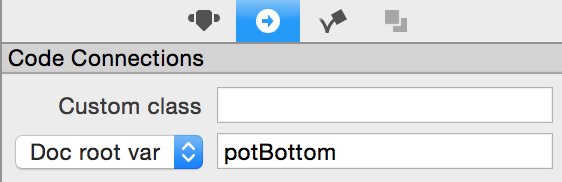
\includegraphics[width=150pt]{images/Chapter6/pot_bottom_code.png}
  \end{figure}
    
  \item Select the \textit{pot-top} node and assign this code connection:
    \begin{figure}[H]
    \centering
    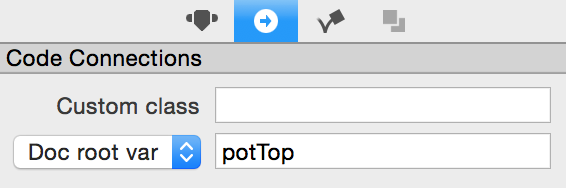
\includegraphics[width=150pt]{images/Chapter6/pot_top_code.png}
  \end{figure}
  
  \item Publish the \SB{} project!
\end{enumerate}
\end{leftbar}

Now we can switch back to \xcode{} and initialize the pot with its correct
z-order values.

First, we need to set up the properties for our code connections.
\begin{leftbar}
Add the following two properties to the \inlinecode{FallingObject} class:
\begin{lstlisting}
weak var potTop: CCNode!
weak var potBottom: CCNode!
\end{lstlisting}
\end{leftbar}

Then we can add the initializer.

\begin{leftbar}
Add this implementation of \inlinecode{didLoadFromCCB} that initializes the
pots' \inlinecode{zOrder} to the \inlinecode{Pot} class:
\begin{lstlisting}
func didLoadFromCCB() {
  potTop.zOrder = DrawingOrder.PotTop.rawValue
  potBottom.zOrder = DrawingOrder.PotBottom.rawValue
}
\end{lstlisting}
\end{leftbar}

Now we need to take care of the falling object. When it is caught, we want to
render it between the two pot parts. For this we need to extend the code that
marks objects as caught.
\begin{leftbar}
Add the relevant line to the \inlinecode{if} case of the
\inlinecode{performFallingStep} method in the \inlinecode{MainScene} class:
\begin{lstlisting}
    ...
      if (// caught) {
        ...
        fallingObject.fallingState = .Caught
        fallingObject.zOrder = Pot.DrawingOrder.FallingObject.rawValue
      }
    ...
\end{lstlisting}
\end{leftbar}
Great! With this tweak we have completed a significant portion of the core
gameplay.

\section{Summary} 
In this chapter we have completed what we call the \textit{core mechanic} of
our game. A player can drag the catching pot across the screen and collect
items.

Along the way you have learned how to incorporate state machines into the
codebase of your game. I hopefully could show that they are a great tool to
structure your gameplay code. 

You have also learnt how to transform node positions
and sizes between different node spaces and how to work with the z-order to
create a 3D feel in a 2D world.

To turn the core mechanic that we have built in this chapter into a game, we
will need to add some rules and game modes. We will tackle that throughout the
next chapter.

\subsection{Grab the Source Code}
You can find the Source Code for this chapter on GitHub:
\url{https://github.com/SpriteBuilder-Book/Code/tree/master/Chapter5/}.
